% Compilar desde esta carpeta; estilo de la clase del jueves 26.
\documentclass[10pt,aspectratio=169,xcolor={dvipsnames}]{beamer}
\usepackage[utf8]{inputenc}
\usepackage[T1]{fontenc}
\usepackage{lmodern}
\usepackage[spanish,es-nodecimaldot]{babel}
\usepackage{amsmath,amssymb,bm}
\usepackage{graphicx,booktabs,tikz,listings}
\usetikzlibrary{arrows.meta,positioning,calc}
\graphicspath{{figuras/}}

% Paleta, títulos y recuadros del material DL_MRI_class.
\definecolor{fondo}{RGB}{18,49,90}
\definecolor{verde}{HTML}{087F6B}
\definecolor{naranja}{HTML}{D65324}
\setbeamercolor{normal text}{fg=fondo,bg=white}
\setbeamercolor{math text}{fg=black!75}
\setbeamercolor{structure}{fg=fondo}
\setbeamercolor{frametitle}{fg=fondo,bg=white}
\setbeamercolor{bottombox}{fg=fondo,bg=white}
\setbeamercolor{lgraybox}{fg=fondo,bg=gray!10}
\setbeamercolor{yellowbox}{fg=fondo,bg=yellow!17}
\setbeamercolor{greenbox}{fg=fondo,bg=verde!10}
\setbeamercolor{orangebox}{fg=fondo,bg=naranja!10}
\setbeamercolor{section title}{fg=fondo,bg=white}
\setbeamercolor{itemize item}{fg=fondo}
\setbeamertemplate{itemize items}[circle]
\setbeamertemplate{navigation symbols}{}
\setbeamersize{text margin left=8mm,text margin right=8mm}
\setbeamertemplate{frametitle}{\vspace{2mm}\color{fondo}\bfseries\insertframetitle\par\vspace{-2mm}\rule{\textwidth}{0.4pt}}
\setbeamertemplate{footline}{%
    \leavevmode\hbox{%
    \begin{beamercolorbox}[wd=.23\paperwidth,ht=2.5ex,dp=1ex,center]{bottombox}
        \insertshortauthor
    \end{beamercolorbox}%
    \begin{beamercolorbox}[wd=.46\paperwidth,ht=2.5ex,dp=1ex,center]{bottombox}
        \insertshorttitle
    \end{beamercolorbox}%
    \begin{beamercolorbox}[wd=.31\paperwidth,ht=2.5ex,dp=1ex,right]{bottombox}
        \insertshortdate\hspace{1.5em}\insertframenumber/\inserttotalframenumber\hspace{2ex}
    \end{beamercolorbox}}\vskip2pt}
\newcommand{\tcg}[1]{\textcolor{verde}{#1}}
\newcommand{\tcr}[1]{\textcolor{naranja}{#1}}
\newenvironment{caja}[1][lgraybox]{\begin{beamercolorbox}[sep=0.7em,wd=\linewidth]{#1}}{\end{beamercolorbox}}
\newcommand{\actividad}[2]{\begin{caja}[yellowbox]\textbf{#1}\par\smallskip #2\end{caja}}
\newcommand{\R}{\mathbb{R}}
\DeclareMathOperator*{\argmin}{arg\,min}
\lstset{language=Python,basicstyle=\ttfamily\small,keywordstyle=\color{fondo}\bfseries,
    commentstyle=\color{verde},stringstyle=\color{naranja},showstringspaces=false,
    columns=fullflexible,keepspaces=true,frame=none,aboveskip=0.5em,belowskip=0.5em}
\setbeameroption{hide notes}
% Para una versión docente intercalada, cambiar la línea anterior por:
% \setbeameroption{show notes}
\AtBeginSection[]{%
    \begin{frame}[plain]
        \vfill
        {\small APRENDIZAJE AUTOMÁTICO INICIAL\par}
        \vspace{5mm}
        {\LARGE\bfseries\insertsection\par}
        \vspace{3mm}{\color{naranja}\rule{0.25\textwidth}{1.2pt}}
        \vfill
    \end{frame}}

\title[Clase 15]{\bfseries Entrenamiento de redes neuronales}
\subtitle{Retropropagación, optimización y generalización}
\author[E. Cueva]{Evelyn Cueva J.}
\institute{Aprendizaje Automático Inicial · Ciencia de Datos}
\date[2 dic. 2026]{Miércoles 2 de diciembre de 2026}

\begin{document}
\begin{frame}[plain]
    \vspace{6mm}{\small CLASE 15\par}\vspace{6mm}
    {\LARGE\bfseries\inserttitle\par}\vspace{3mm}
    {\color{fondo}\rule{0.92\textwidth}{1pt}}\par
    {\large\insertsubtitle\par}\vspace{8mm}
    \insertauthor\par\smallskip{\small\insertinstitute\par}\vspace{3mm}
    {\small\insertdate\par}\vfill
\end{frame}
\begin{frame}{Una red con muchos parámetros: ¿cómo ajustarlos?}
\begin{itemize}
\item El jueves: una neurona y descenso del gradiente.
\item El lunes: salidas y pérdidas para clasificación.
\item El martes: composición de capas para relaciones no lineales.
\end{itemize}\begin{caja}[yellowbox]
Hoy: calcular los gradientes de toda la red y aprender sin memorizar los datos.
\end{caja}

\note{}
\end{frame}

\begin{frame}{Objetivos y recorrido}
\begin{itemize}
\item Deducir retropropagación con la regla de la cadena.
\item Distinguir cálculo de gradientes y actualización de parámetros.
\item Comparar SGD, momentum, RMSProp y Adam.
\item Relacionar validación, regularización y parada temprana.
\end{itemize}
\note{}
\end{frame}

\section{Retropropagación: derivar una composición}
\begin{frame}{Dos recorridos por la misma red}
\centering
\begin{tikzpicture}[>=Latex,node distance=6mm,
paso/.style={draw=fondo,rounded corners,fill=fondo!5,minimum height=10mm,text width=18mm,align=center}]
\node[paso] (x) {Entrada\\$\bm x$};
\node[paso,right=of x] (h) {Oculta\\$\bm h$};
\node[paso,right=of h] (p) {Predicción\\$\hat{\bm y}$};
\node[paso,right=of p] (l) {Pérdida\\$\mathcal L$};
\draw[->,thick,verde] (x)--(h);\draw[->,thick,verde] (h)--(p);\draw[->,thick,verde] (p)--(l);
\draw[->,thick,naranja] (l.south)--++(0,-0.7)-|(h.south);
\node[text=naranja] at (3.9,-1.35) {Hacia atrás: regla de la cadena};
\end{tikzpicture}\par\bigskip\raggedright
\textbf{Forward pass:} calcula activaciones y pérdida.\par\medskip
\textbf{Backward pass:} calcula derivadas respecto a los parámetros.
\par\medskip\textbf{Optimizador:} usa esas derivadas para actualizar los parámetros.
\note{}
\end{frame}

\begin{frame}{Un ejemplo pequeño que podemos derivar completo}

Una entrada, una neurona oculta ReLU y una salida lineal:
\[z=wx+b,\quad h=\max(0,z),\quad\hat y=vh+c,
\quad\ell=\tfrac12(\hat y-y)^2.\]
\begin{caja}[yellowbox]
Dato: $x=2$, $y=3$. Parámetros: $w=1$, $b=0$, $v=0.5$, $c=0$.
\end{caja}
\[z=2,\quad h=2,\quad\hat y=1,\quad\ell=2.\]
El factor $1/2$ simplifica la derivada de este ejemplo; no es la convención del MSE de Keras.
\note{}
\end{frame}

\begin{frame}{Primero: derivar la salida}

\[\delta_{\rm salida}=\frac{\partial\ell}{\partial\hat y}=\hat y-y=-2.\]
Como $\hat y=vh+c$:
\[\frac{\partial\ell}{\partial v}=\delta_{\rm salida}h=-4,
\quad\frac{\partial\ell}{\partial c}=\delta_{\rm salida}=-2,
\quad\frac{\partial\ell}{\partial h}=\delta_{\rm salida}v=-1.\]
\begin{caja}[greenbox]La derivada hacia la capa anterior se obtiene multiplicando por el peso de la conexión.\end{caja}
\note{}
\end{frame}

\begin{frame}{Después: atravesar la activación y llegar a la entrada}

\[\operatorname{ReLU}'(z)=\begin{cases}1,&z>0,\\0,&z<0.\end{cases}\]
Aquí $z=2>0$, por tanto:
\[\delta_{\rm oculta}=\frac{\partial\ell}{\partial z}
=\frac{\partial\ell}{\partial h}\operatorname{ReLU}'(z)=-1.\]
\[\frac{\partial\ell}{\partial w}=\delta_{\rm oculta}x=-2,
\qquad\frac{\partial\ell}{\partial b}=\delta_{\rm oculta}=-1.\]
\actividad{Piensa}{Si $z<0$, ¿qué pasaría con los gradientes de $w$ y $b$ en este ejemplo?}
\note{ReLU no es diferenciable en cero; los frameworks adoptan una convención para ese punto. Si una unidad permanece en la zona negativa para todos los datos, puede dejar de aprender por esta ruta.}
\end{frame}

\begin{frame}{Un paso con todos los gradientes calculados}

Con $\eta=0.1$ y usando los parámetros anteriores en todas las derivadas:
\[w'=1.2,\quad b'=0.1,\quad v'=0.9,\quad c'=0.2.\]
Nueva pasada hacia adelante:
\[z'=2.5,\quad h'=2.5,\quad\hat y'=2.45,
\quad\ell'=\tfrac12(2.45-3)^2=0.15125.\]
\begin{caja}[greenbox]Retropropagación calcula gradientes; descenso del gradiente actualiza parámetros.\end{caja}
No sustituimos pesos recién actualizados dentro de la misma pasada hacia atrás.
\note{}
\end{frame}

\begin{frame}{La misma idea para muchas capas}

\[\bm a^{(0)}=\bm x,\quad
\bm z^{(l)}=(W^{(l)})^\top\bm a^{(l-1)}+\bm b^{(l)},
\quad\bm a^{(l)}=\sigma_l(\bm z^{(l)}).\]
\[\bm\delta^{(l)}=
\bigl(W^{(l+1)}\bm\delta^{(l+1)}\bigr)\odot\sigma'_l(\bm z^{(l)}).\]
\[\frac{\partial\ell}{\partial W^{(l)}}=
\bm a^{(l-1)}(\bm\delta^{(l)})^\top,
\qquad \frac{\partial\ell}{\partial\bm b^{(l)}}=\bm\delta^{(l)}.\]
$\odot$: producto componente a componente. Para un lote, promediamos sus gradientes.
\note{Convención: W de dimensión n_anterior por n_actual y vectores columna. Para BCE+sigmoide o CE+softmax, delta de salida es p-y por observación. La recurrencia escrita supone activaciones ocultas componente a componente; no sustituir la derivada de softmax por una derivada escalar.}
\end{frame}

\begin{frame}{Gradientes pequeños: una dificultad de las composiciones}
\begin{itemize}
\item La regla de la cadena multiplica derivadas de varias capas.
\item Muchas derivadas pequeñas pueden hacer muy pequeño el gradiente de las primeras capas.
\item Revisar escalas de entrada, inicialización y activaciones antes de aumentar épocas.
\end{itemize}
\note{La sigmoide tiene derivada máxima 1/4; cadenas largas pueden atenuar el gradiente. No afirmar que ReLU elimina todos los problemas de gradiente. También puede haber gradientes explosivos.}
\end{frame}

\section{Optimización: cómo usar los gradientes}
\begin{frame}{SGD y lotes: recordar qué cuenta como un paso}

\[\bm g_t=\frac1{|B_t|}\sum_{i\in B_t}\nabla_{\bm\theta}\ell_i,
\qquad\bm\theta_{t+1}=\bm\theta_t-\eta\bm g_t.\]
\begin{caja}
\textbf{Epoch:} recorrer el entrenamiento una vez.
\textbf{Batch size:} número de observaciones por lote.
\textbf{Update:} modificar parámetros tras calcular el gradiente de un lote.
\end{caja}
Con 30 datos y lotes de 10: tres actualizaciones por época.
La aleatoriedad de los minilotes puede introducir fluctuaciones en el descenso.
\note{}
\end{frame}

\begin{frame}{Momentum: acumular una dirección}

\[\bm v_t=\mu\bm v_{t-1}-\eta\bm g_t,\qquad
\bm\theta_{t+1}=\bm\theta_t+\bm v_t.\]
\begin{caja}[greenbox]
El paso combina el gradiente actual con parte del desplazamiento anterior.
\end{caja}
Puede reducir oscilaciones y sostener avance en direcciones consistentes.
\par\medskip En el notebook: SGD con tasa 0.01 y momentum 0.9.
\note{Esta es la convención de velocidad con tasa incluida. Otras fuentes guardan promedios de gradientes y escriben fórmulas equivalentes con otra escala. No comparar sin identificar la convención.}
\end{frame}

\begin{frame}{RMSProp: adaptar la escala por parámetro}

\[\bm s_t=\rho\bm s_{t-1}+(1-\rho)\bm g_t\odot\bm g_t,\]
\[\bm\theta_{t+1}=\bm\theta_t-
\eta\frac{\bm g_t}{\sqrt{\bm s_t}+\epsilon}.\]
\begin{caja}Mantiene un promedio de gradientes al cuadrado para ajustar la escala de cada componente del paso.\end{caja}
Las operaciones son componente a componente; $\epsilon$ evita dividir por cero.
\note{Fórmula conceptual: la ubicación exacta de epsilon puede variar por implementación. La tasa global sigue siendo un hiperparámetro; adaptar escalas no garantiza un mínimo global.}
\end{frame}

\begin{frame}{Adam: combinar dirección y escala adaptativa}

\[\bm m_t=\beta_1\bm m_{t-1}+(1-\beta_1)\bm g_t,\qquad
\bm s_t=\beta_2\bm s_{t-1}+(1-\beta_2)\bm g_t^2.\]
Con estados iniciales cero, corregimos el sesgo inicial:
\[\hat{\bm m}_t=\frac{\bm m_t}{1-\beta_1^t},\quad
\hat{\bm s}_t=\frac{\bm s_t}{1-\beta_2^t},\quad
\bm\theta_{t+1}=\bm\theta_t-\eta\frac{\hat{\bm m}_t}{\sqrt{\hat{\bm s}_t}+\epsilon}.\]
\begin{caja}[yellowbox]Adam adapta el paso, pero todavía necesita una tasa de aprendizaje y validación.\end{caja}
\note{Cuadrado, raíz y división componente a componente. Fórmula pedagógica de Adam; detalles de epsilon pueden variar por implementación. No asumir que Adam siempre supera SGD.}
\end{frame}

\begin{frame}{Comparar optimizadores con un protocolo común}
\begin{itemize}
\item Mismos datos, partición, arquitectura y pesos iniciales.
\item Mismo tamaño de lote y presupuesto de actualizaciones; repetir con varias semillas.
\item Ajustar tasas con validación; no exigir una tasa idéntica para todos los métodos.
\item Comparar pérdida de validación, estabilidad y tiempo, además de la pérdida de entrenamiento.
\end{itemize}
\note{Notebook 15, parte 4: SGD con momentum, Adam y RMSprop. Las tasas originales son 0.01, 0.001 y 0.001. No describir la comparación como un experimento donde solo cambió el nombre del optimizador.}
\end{frame}

\section{Generalización: aprender sin memorizar}
\begin{frame}{Sobreajuste: entrenamiento y validación se separan}
\centering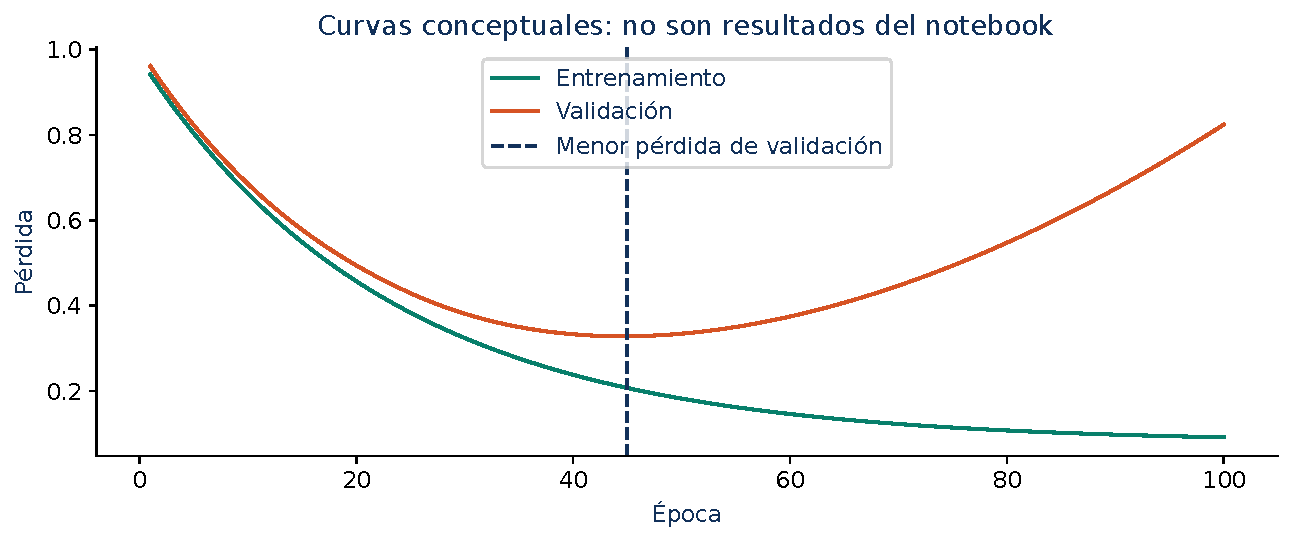
\includegraphics[width=\linewidth,height=4cm,keepaspectratio]{sobreajuste.pdf}\par\medskip
aggedright\small Las curvas son conceptuales. La mejor época de validación puede ocurrir antes de la menor pérdida de entrenamiento.
\note{}
\end{frame}

\begin{frame}{L1 y L2: penalizar pesos grandes}

\[\mathcal J(\bm\theta)=\mathcal L_{\rm datos}(\bm\theta)+\lambda R(W).\]
\begin{columns}[T]
\begin{column}{0.47\textwidth}\begin{caja}
\textbf{L1:} $R(W)=\sum_j|w_j|$.\par\medskip
Favorece soluciones con pocos pesos distintos de cero.
\end{caja}\end{column}
\begin{column}{0.47\textwidth}\begin{caja}
\textbf{L2:} $R(W)=\sum_jw_j^2$.\par\medskip
Penaliza especialmente pesos grandes; derivada $2\lambda W$.
\end{caja}\end{column}
\end{columns}
\medskip $\lambda$ se elige con validación; regularizar demasiado puede causar subajuste.
\note{En Keras kernel_regularizer actúa sobre la matriz de pesos de la capa, no por defecto sobre el sesgo. L1 no garantiza ceros exactos con cualquier optimizador. Al comparar loss con y sin regularización, distinguir penalización incluida y pérdida de datos.}
\end{frame}

\begin{frame}{Dropout: variar las rutas durante el entrenamiento}

\[m_j\sim\operatorname{Bernoulli}(1-q),\qquad
\tilde h_j=\frac{m_jh_j}{1-q}.\]
\begin{caja}[greenbox]
Con tasa $q=0.3$, se enmascaran al azar activaciones durante el entrenamiento.
No se eliminan permanentemente las neuronas.
\end{caja}
En inferencia no se aplica esta máscara. La escala anterior preserva la activación esperada.
\actividad{Interpreta}{¿Por qué la pérdida durante entrenamiento puede ser mayor que en validación?}
\note{Dropout y otras diferencias entre modo entrenamiento e inferencia pueden explicarlo; también revisar cómo se promedian las métricas. No concluir que siempre ocurre ni que cualquier diferencia se debe a dropout.}
\end{frame}

\begin{frame}[fragile]{Early stopping: decidir cuándo detenerse}
\begin{lstlisting}
early = EarlyStopping(
    monitor="val_loss", patience=20,
    restore_best_weights=True)
history = model.fit(
    X_train, y_train, validation_data=(X_val, y_val),
    epochs=200, batch_size=32, callbacks=[early])
\end{lstlisting}
\begin{caja}[greenbox]
Paciencia: número de épocas sin mejora antes de parar. Se restauran los pesos de la mejor época observada.
\end{caja}

\note{Se monitorea validación, nunca el test. La parada ocurre después de la mejor época por la paciencia; no confundir la línea de detención con el mínimo. El criterio exacto también depende de min_delta y mode.}
\end{frame}

\begin{frame}{Notebook 15: un experimento por técnica}
\begin{itemize}
\item Datos: las seis variables del caso Pokémon y su clase Stage.
\item Separar 60/20/20 antes de ajustar StandardScaler; estratificar.
\item Comparar baseline, L2, dropout y early stopping manteniendo el resto fijo.
\item En la parte de optimizadores, conservar arquitectura e inicialización.
\item Evaluar una sola vez en prueba después de elegir con validación.
\end{itemize}
\note{El notebook original ajusta StandardScaler antes de dividir: aplicar la corrección descrita en la guía docente. Las celdas 16 a 26 definen y entrenan las variantes; las celdas 32 a 36 comparan optimizadores. No hay una ejecución manual de backprop en el original: usar el ejemplo de estas diapositivas.}
\end{frame}

\begin{frame}[fragile]{Una capa regularizada en Keras}
\begin{lstlisting}
model = Sequential([
    Input(shape=(6,)),
    Dense(64, activation="relu",
          kernel_regularizer=l2(0.01)),
    Dropout(0.3),
    Dense(32, activation="relu"),
    Dense(3, activation="softmax")
])
model.compile(optimizer=Adam(learning_rate=0.001),
              loss=CategoricalCrossentropy(),
              metrics=["accuracy"])
\end{lstlisting}

\note{Ejemplo de sintaxis combinada; para atribuir efectos, comenzar probando L2 y dropout por separado. Importaciones en notebook 15. Etiquetas one-hot de tres clases.}
\end{frame}

\begin{frame}{Diagnóstico antes de cambiar toda la red}
\small
\begin{tabular}{p{0.40\textwidth}p{0.52\textwidth}}\toprule
Observación & Qué revisar\\\midrule
Entrenamiento y validación altos & Capacidad, escalado, tasa, errores en los datos\\[2mm]
Entrenamiento baja, validación sube & Sobreajuste; regularización y parada temprana\\[2mm]
Pérdida oscila o diverge & Tasa excesiva, escalas o gradientes\\[2mm]
Gradientes casi nulos & Saturación, inicialización y profundidad\\\bottomrule
\end{tabular}\par\bigskip
Son hipótesis de diagnóstico, no conclusiones automáticas.
\note{}
\end{frame}

\begin{frame}{Cierre: explicar el ciclo completo}
\begin{itemize}
\item La pasada hacia adelante produce predicciones y pérdida.
\item Retropropagación aplica la regla de la cadena para calcular gradientes.
\item El optimizador transforma los gradientes en actualizaciones.
\item La validación orienta decisiones; la regularización controla el sobreajuste.
\item La prueba estima el desempeño final en datos reservados.
\end{itemize}\begin{caja}[yellowbox]
Pregunta final: ¿por qué una pérdida de entrenamiento menor no garantiza un mejor modelo?
\end{caja}

\note{}
\end{frame}

\end{document}
